%!TEX root = ../draft.tex
\chapter{Umsetzung}
Das Anforderungsmanagement teilt sich in mehrere Abschnitte ein, jeder dieser Abschnitte stellt einen wichtigen Prozess für den Umgang mit Anforderungen dar. Der erste Schritt ist die \nameref{sec:ermittlung}, wobei die Anforderungen der Stakeholder ermittelt werden, um sie daraufhin zu dokumentieren. Ist die \nameref{sec:dokumentation} abgeschlossen, folgt die \nameref{sec:auswertung} der dokumentierten Anforderungen. Bei einem agilen Projekt wie es das \ac{LWM} darstellt, wird dieser Vorgang in Iterationen bis zu einem beliebigen Detailgrad immer wieder verfeinert.

\section{Ermittlung}
\label{sec:ermittlung}

Aus der Problemstellung ist zu entnehmen, dass nicht das Ermitteln neuer ausgefallener Ideen und Features das Ziel ist, sondern das in Erfahrung bringen der Wünsche und Voraussetzungen der Stakeholder. In anderen Worten: Es wird das Ziel verfolgt Basis- und Leistungsfaktoren zu ermitteln. Aus diesem Grund wurde bewusst Abstand von den in Kapitel \ref{subsubsec:kreativitätstechniken} beschriebenen Kreativitätstechniken genommen. Auch wurde sich gegen die in Kapitel \ref{subsubsec:fragebogen} aufgeführten Fragebogen-Methode entschieden, da die befragten Stakeholder dazu nicht über genügende Kenntnisse über das Produkt verfügten.\\

Unter anderem aus diesem Grund, etablierte sich die \nameref{subsubsec:interview}-Technik. Bei dieser Technik geht es darum, ein Interview über vorbereitete und vorformulierte Fragen mit den gewählten Stakeholdern zu führen. So ist es möglich, während dem Gespräch auftretende Fragen direkt zu klären und somit auch implizite Anforderungen aufzudecken. Zudem öffnet diese Methode die Tür für neue Anforderungen oder Problemstellungen, welche bislang nicht in Betracht gezogen wurden. 
Ein weiterer Vorteil dieser Technik ist, dass die Hemmungen der Stakeholder durch ein offenes Gespräch gelindert werden.\\

Zu Beginn der Ermittlung wurde ein zweiseitiger Fragebogen (siehe Anhang \ref{anh:fragebogen}) als Leitfaden für die Interviews erstellt, welcher in kurzen Stichpunkten die wesentlichen Problemstellungen und Platz für die darauf bezogenen Notizen beinhaltet. Die dort aufgeführten Probleme beruhen auf Erfahrungen mit dem bestehenden Tool und wurden durch  \nameref{subsubsec:brainstorming} ergänzt. 
Mit diesem Formular konnte nicht nur der Umgang mit den bekannten Problemen des Tools, sondern auch solche, die aus Ausnahmesituationen resultieren, zur Sprache gebracht werden.\\

Im Anschluss daran wurde mit Hilfe des Entwickler-Teams, sowohl Frontend als auch Backend, eine Eingrenzung der Stakeholder vorgenommen. Dieser ausgewählte Kreis wurde per E-Mail kontaktiert und um einen Gesprächstermin gebeten, sofern Interesse an der Nutzung eines Tools zu Verwaltung der Praktika besteht. \\

Bei dem Ablauf der Interviews ist grundsätzlich zwischen den aktuellen Nutzern und den potentiell zukünftigen Nutzern zu unterscheiden. Zwar wurde das Ziel verfolgt, losgelöst von dem aktuellen Tool über ein "Wunschsystem" zu sprechen, jedoch war dies einerseits bei den bestehenden Nutzern kaum möglich, da diese sich instinktiv immer wieder an dem derzeitigen Tool orientierten. Andererseits konnte dieses bei den Stakeholdern, für die dieses System zu diesem Zeitpunkt noch unbekannt war, als perfekte Beschreibung der Thematik genutzt werden.\\

Ein Interview begann, sofern erforderlich, mit der Beschreibung des bestehenden Tools, um eine Ausgangsgrundlage für das Gespräch zu schaffen. Nach der Darlegung der Problemstellung war jedem Gesprächspartner der Hintergrund dieser Anforderungsermittlung bekannt. Mit der Aufforderung, zunächst vollkommen losgelöst von den vorgefertigten Fragen, den Ablauf des Praktikums und dessen Bewertung zu erklären, konnten zu diesem Zeitpunkt schon eine Vielzahl dieser Fragen beantwortet werden. Diese Informationen wurden durch Fragen mit einem "Was wäre wenn"-Stil ergänzt, wobei zu beachten war, dass die Gesprächspartner nicht in eine vorgegebene Denkweise geleitet werden. So wurden auch kleinste Probleme, die bei der Nutzung eines solchen Tools auftreten können, aufgedeckt und dokumentiert.\\

Die Anforderungen der Nutzer wurden während des Gesprächs bestmöglich in die Kano-Faktoren eingeteilt, welche in Kapitel \ref{sec:kano} beschrieben wurden. Dadurch konnte eine grobe Priorisierung nach \textit{Basisfaktoren}, \textit{Leistungsfaktoren} und \textit{Begeisterungsfaktoren} schon vor der eigentlichen Auswertung vorgenommen werden.\\

Durch die Interviews konnten über 150 Anforderungen ermittelt werden, wovon einige durch das gegenwärtige Tool schon abgedeckt werden und andere, welche eine ganz neue Perspektive auf das System und dessen Möglichkeiten ermöglichen.


\section{Zielgruppe}

Als Stakeholder ist grundsätzlich jeder zu betrachten, der aktiv an dem Tool oder dessen Nutzung beteiligt ist oder durch diese beeinflusst wird. Durch diese Definition befinden sich in der Gruppe der Stakeholder nicht nur das Entwickler-Team, sondern auch Studenten, Administratoren, Modulverantwortliche, Mitarbeiter, \ac{SHK} und \ac{WHK}. \\[1em]

Die Anforderungsermittlung über Studenten wurde nicht in Betracht gezogen, da dies nicht in den zeitlichen Rahmen dieser Arbeit gepasst hätte. Zudem sind Studenten zwar direkte Nutzer des Systems, jedoch arbeiten sie, im Gegensatz zu den anderen Stakeholdern, verhältnismäßig wenig damit.\\
Die Anforderungen des Entwickler-Teams wurden, im Laufe der Anforderungsauswertung  und Validation, aufgenommen.\\
Von den verbleibenden Stakeholdern erwies es sich als sinnvoll, die Modulverantwortlichen als Interessenvertreter anzusehen.\\[1em]

Durch das Modulhandbuch des Campus konnte eine Liste der existierenden Module erstellt werden. Die Email-Adressen der Modulverantwortlichen konnte von der Webseite der TH-Köln bezogen werden.\\
Mit der Vorgabe den Kreis der Nutzer auf den Bereich des Instituts für Informatik zu begrenzen, beinhaltet diese Liste 61 Module.\\

Durch ein Gespräch mit dem Entwickler-Team, konnte diese Liste anschließend auf circa 20 Module begrenzt werden, indem die Module, die kein Praktikum veranstalten, aussortiert wurden.\\

Nach der Kontaktierung der jeweiligen Modulverantwortlichen, bestätigten 14 von diesen ein Interesse an diesem Projekt und erklärten sich zu einem Interview bereit.

\section{Dokumentation}
\label{sec:dokumentation}

\subsection{Formulierung}

Um die auf den Interview-Bögen notierten Anforderungen, mit allen nötigen Details, zu dokumentieren, wurde auf eine abgewandelte Form der in Kapitel \ref{subsec:functionmaster} erläuterten Schablone zurückgegriffen. \\

In einer etwas angepassten Form sieht der Satzbau wie folgt aus:\\

\textit{<Zielsystem> <Priorität>} einem \textit{<Stakeholder>} die Möglichkeit bieten, \textit{<Funktion>}.\\

Erklärung:
\begin{description}
\item \textit{<Zielsystem>}

Das Zielsystem stellt das referenzierte System dar. Hierbei steht \textit{"Das bestehende System"} für das aktuelle \ac{LWM} und \textit{"Das zu entwickelnde System"} für ein neues System . Die Unterscheidungen dieser Systeme wird in Kapitel \ref{sec:auswertung} genauer erläutert. 

\item \textit{<Priorität>}

Hier wird mit Hilfe des Kano-Modell von Prof. Noriaki Kano priorisiert. Für einen Basis-Faktor wird, mit Anlehnung an \cite{Rupp14}, das Schlüsselwort \textit{"muss"}, für einen Leistungs-Faktor \textit{"soll"} und für einen Begeisterungsfaktor \textit{"wird"} eingesetzt. 

\item \textit{<Stakeholder>}

Hier wird die Liste von Stakeholdern, welche von dieser Anforderung Gebrauch machen würden eingesetzt.

\item \textit{<Funktion>}

Die Funktion beschreibt den eigentlichen Sinn dieser Anforderung.

\end{description}

Ein Beispiel aus dieser Arbeit sieht wie folgt aus:\\

\textit{"Das bestehende System soll einem Modulverantwortlichen und einem Mitarbeiter die Möglichkeit geben, eine gelbe Karte für eine unbefriedigende Abgabe zu erteilen."}\\

oder:\\

\textit{"Das zu entwickelnde System wird einem Modulverantwortlichen, einem Mitarbeiter, einer Studentischen Hilfskraft und einem Studenten die Möglichkeit geben, Termine in einer gegebenen Frist zu stornieren."}

\section{Auswertung}
\label{sec:auswertung}

Für die Arbeit mit den Anforderungen, ist es notwendig, diese auszuwerten.
Das \ac{LWM} ist ein agiles Projekt, weshalb es sinnvoll war, auch die Anforderungsauswertung diesem Stil entsprechend durchzuführen. Hierzu wurden die Anforderungen nach der \nameref{subsec:validation} in einer Art Epic zusammengefasst. Anschließend wurden diese Gruppen priorisiert. Hier setzt ein neuer Iterationsschritt ein, indem eine Gruppe mit der höchsten Priorität selektiert und wiederum in Untergruppen eingeteilt wurde. Diese Untergruppen konnten anschließend wieder priorisiert werden. Dieser Vorgang kann je nach Belieben wiederholt werden. Ist der gewünschte Detailgrad erreicht, fällt es leicht die Komplexität der einzelnen Anforderungen zu schätzen.


\subsection{Validation}
\label{subsec:validation}
Der erste Schritt in der Auswertung war die Validation. Die Anforderungen wurden für ein schon bestehendes System aufgenommen, weshalb es vorkommen kann, dass Anforderungen schon erfüllt wurden. Um die spätere Verarbeitung zu vereinfachen, wurde deshalb im Vorfeld eine Validation der Anforderungen vorgenommen. Hierbei wurden diese in drei Kategorien aufgeteilt. Es wurde unterschieden zwischen \textit{"Erledigt"}, \textit{"Valide"} und \textit{"Verworfen"}. Die Anforderungen aus den Kategorien \textit{"Erledigt"} und \textit{"Verworfen"} werden zwar nicht gelöscht, da diese auch während der Implementierung von anderen Anforderungen von Relevanz sein können, jedoch werden diese bei der Priorisierung nicht beachtet. Auch gibt es für diese Anforderungen im ersten Moment keine Aufwandsschätzung, da diese derzeit keinen Aufwand bedeuten.

\subsection{Gruppierung}

Eine unsortierte Liste von Anforderungen kann nicht so einfach ausgewertet werden, weshalb ein Verfahren gefunden werden muss, diese Anforderungen in kleinere Gruppen zu sortieren. Mit diesen Gruppen fällt nicht nur die Übersicht leichter, sondern auch die spätere Priorisierung und Aufwandsschätzung.\\

Im Laufe der Anforderungsermittlung wurde deutlich, dass einige Anforderungen die eigentliche Grenze des aktuellen \ac{LWM} überschreiten. So wurde beispielsweise ein Forum für das Besprechen von Problemstellungen gefordert, was jedoch nicht direkt mit der Praktikumsverwaltung selbst zu tun hat. Da diese Ideen jedoch nicht verworfen werden sollen, da sie einen Mehrwert für den Praktikumsverlauf darstellen, wurde mit dem Entwickler-Team die Entscheidung getroffen, die Anforderungen aufzuteilen. Die erste Gruppierung erfolgte somit durch die Unterscheidung, ob eine Anforderung einem neuen System, oder dem bestehenden System zuzuordnen ist.\\

Des Weiteren wurde sich für eine Gruppierung nach Aufgabengebiet entschieden. Dies ist ein sehr grobes Verfahren, was allerdings in Anbetracht der Menge von Anforderungen, als angemessen empfunden wurde. Ganz nach dem Prinzip \texttt{divide and conquer} wurden erst wenige große Gruppen erstellt, die anschließend durch weitere Iterationen verfeinert werden. \\

Eine Möglichkeit Anforderungen in einer höheren Abstraktionsebene zu beschreiben sind Epics. Epics beschreiben eine Masse an Anforderungen mit einer User-Story. Auch wenn das Prinzip von Epics in diesem Anwendungsfall verfolgt wurde, fiel die Entscheidung gegen die Beschreibung in Form einer User-Story, da dies auf diesem Abstraktionslevel nicht angebracht war. Ab einem gewissen Detailgrad ist dies jedoch durchaus sinnvoll.\\

Diese Gruppierung erfolgte durch die Aufteilung in Aufgabengebiete an einem Whiteboard. 
\begin{figure}[!htb]
		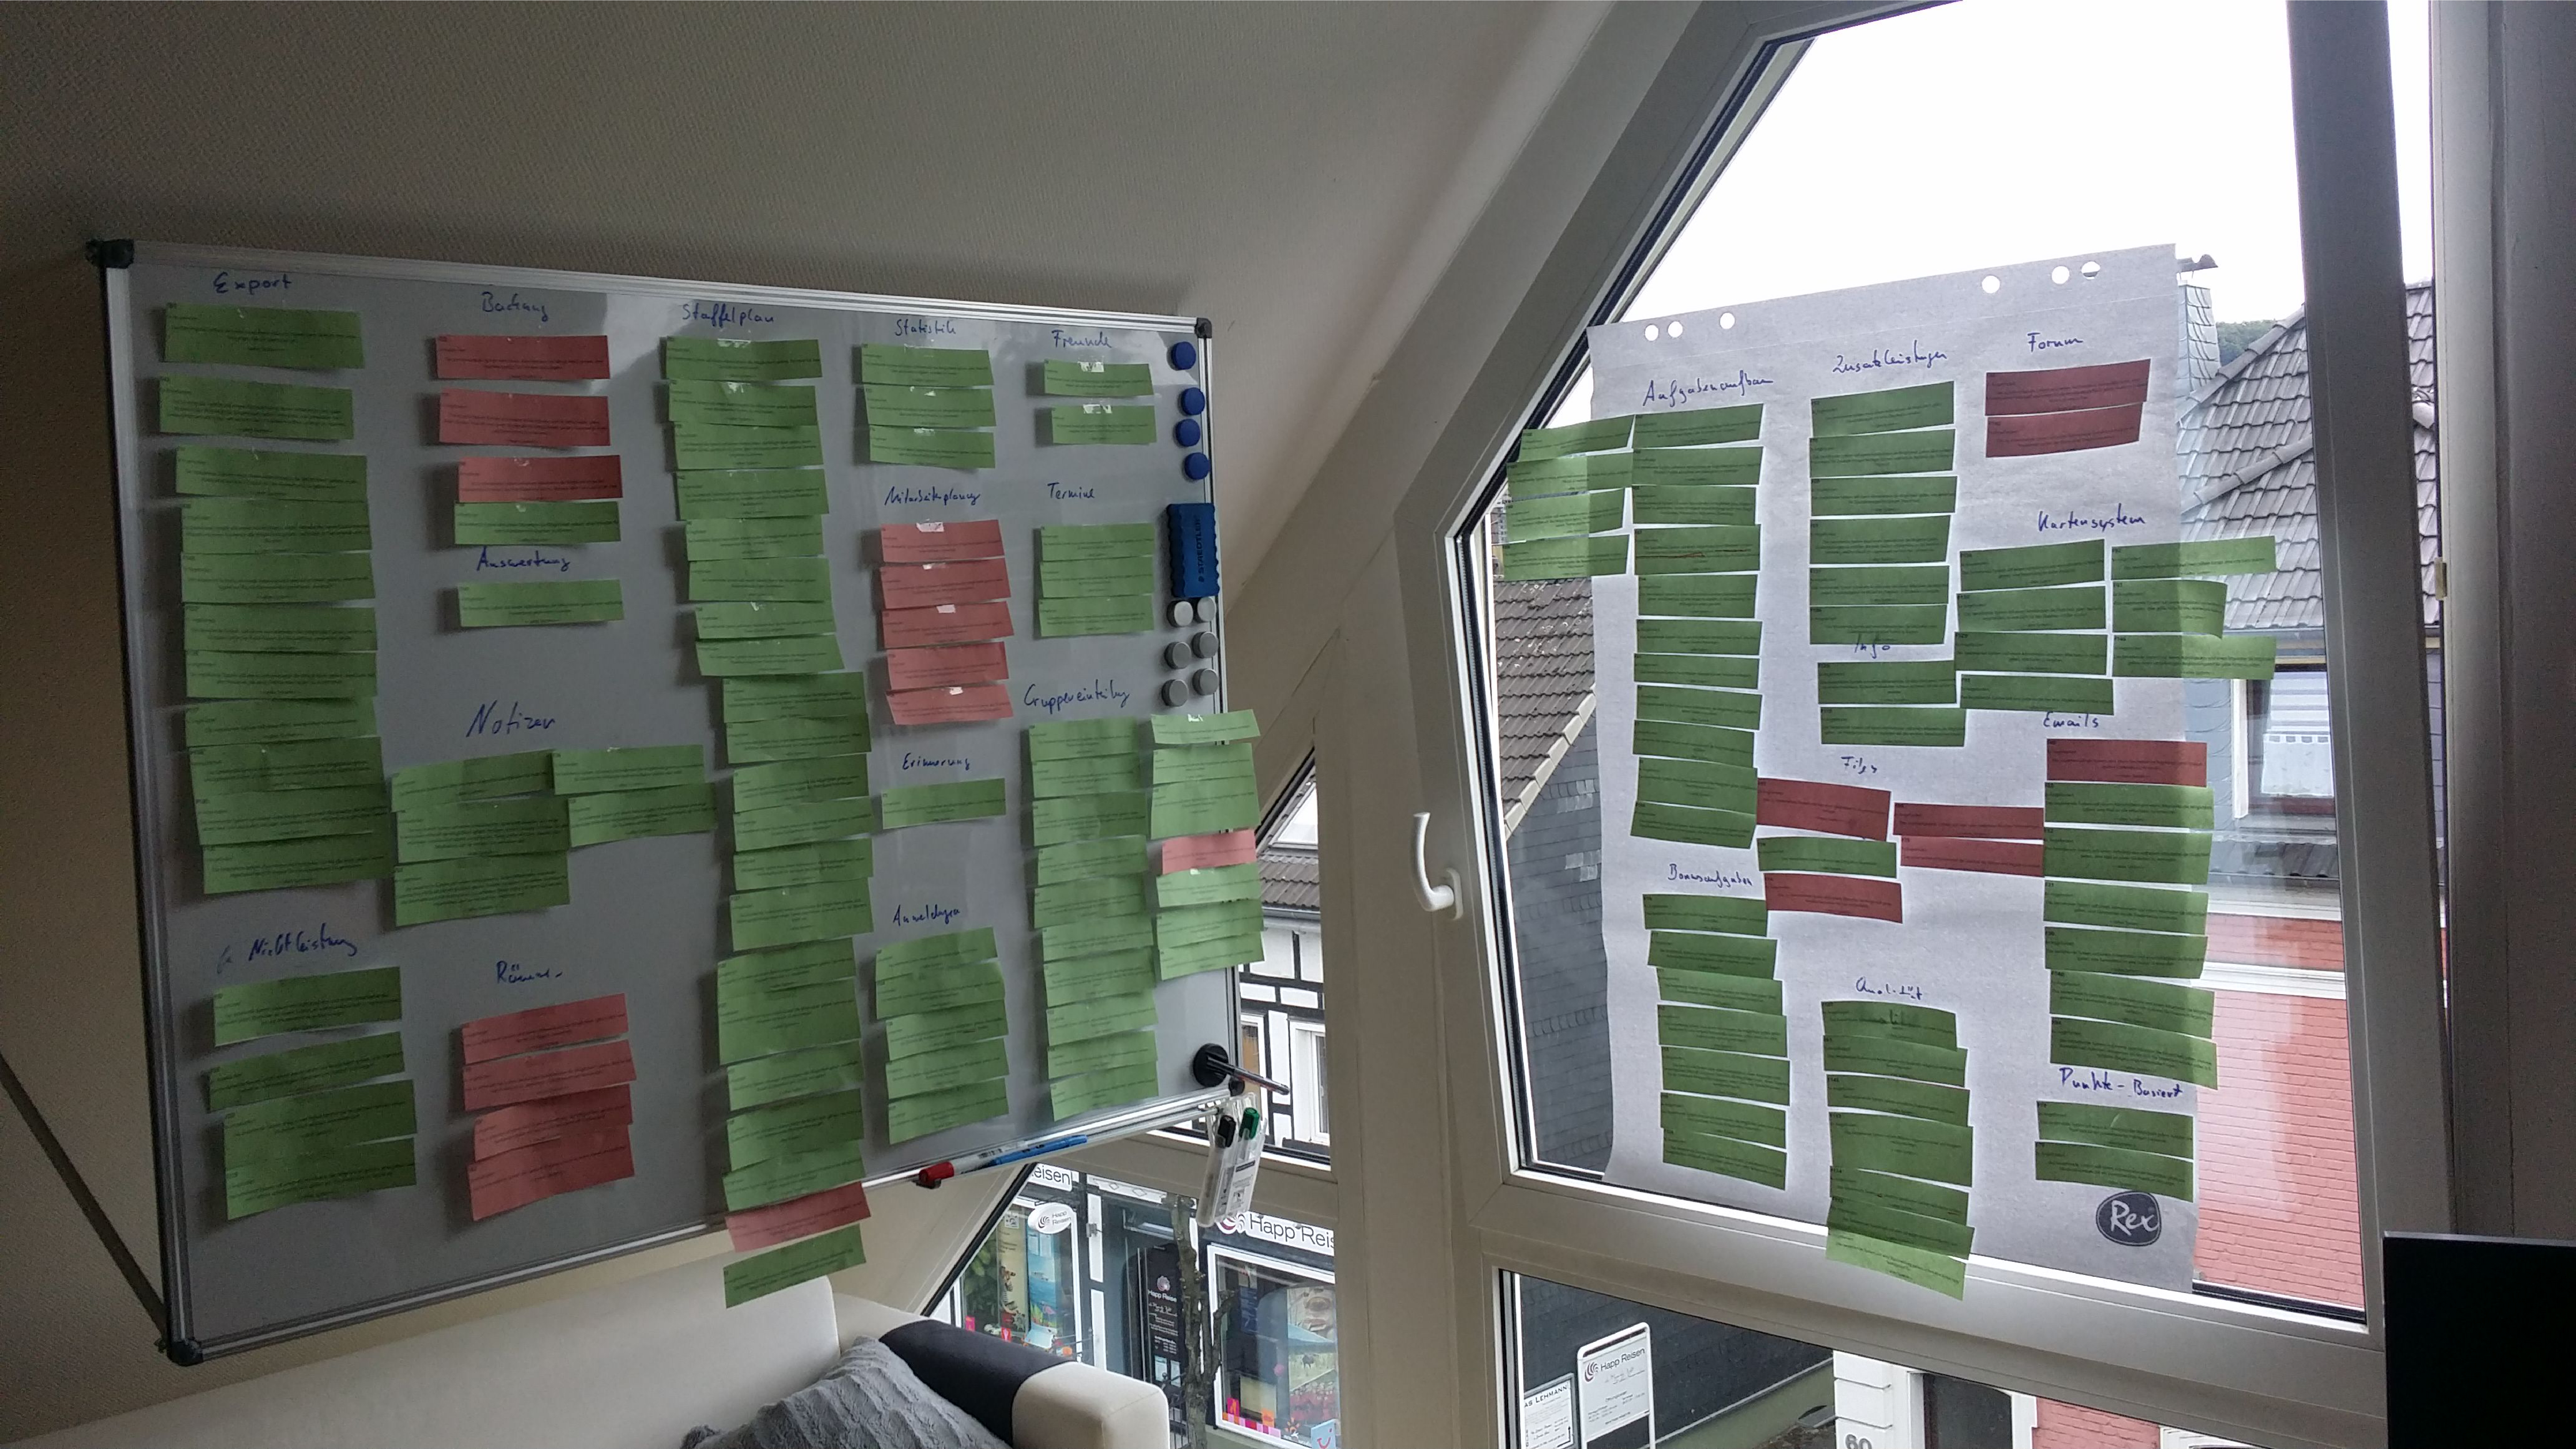
\includegraphics[width=\textwidth]{images/erstegruppen.pdf}
\centering 
\captionabove[Gruppeneinteilung zweiter Ebene]{Gruppeneinteilung zweiter Ebene\footnotemark} 
\end{figure}
\footnotetext{Ein Bild von der Gruppeneinteilung auf zweiter Ebene an einem Whiteboard} 

So konnten die circa 150 Anforderungen in 24 Gruppen eingeteilt werden.\\

Nach der ersten Priorisierung, auf welche in Kapitel \ref{subsec:priorisierung} näher eingegangen wird, wurde zunächst die Gruppe mit der höchsten Priorität ausgewählt, um sie in kleinere Einheiten zu zerlegen. Dies erfolgte in einem Meeting gemeinsam mit dem Entwickler-Team. Hierzu wurden die Anforderungen der Gruppe \textit{"Staffelplan"} auf einem Whiteboard in eine Ablaufreihenfolge gebracht. 

\begin{figure}[!htb]
		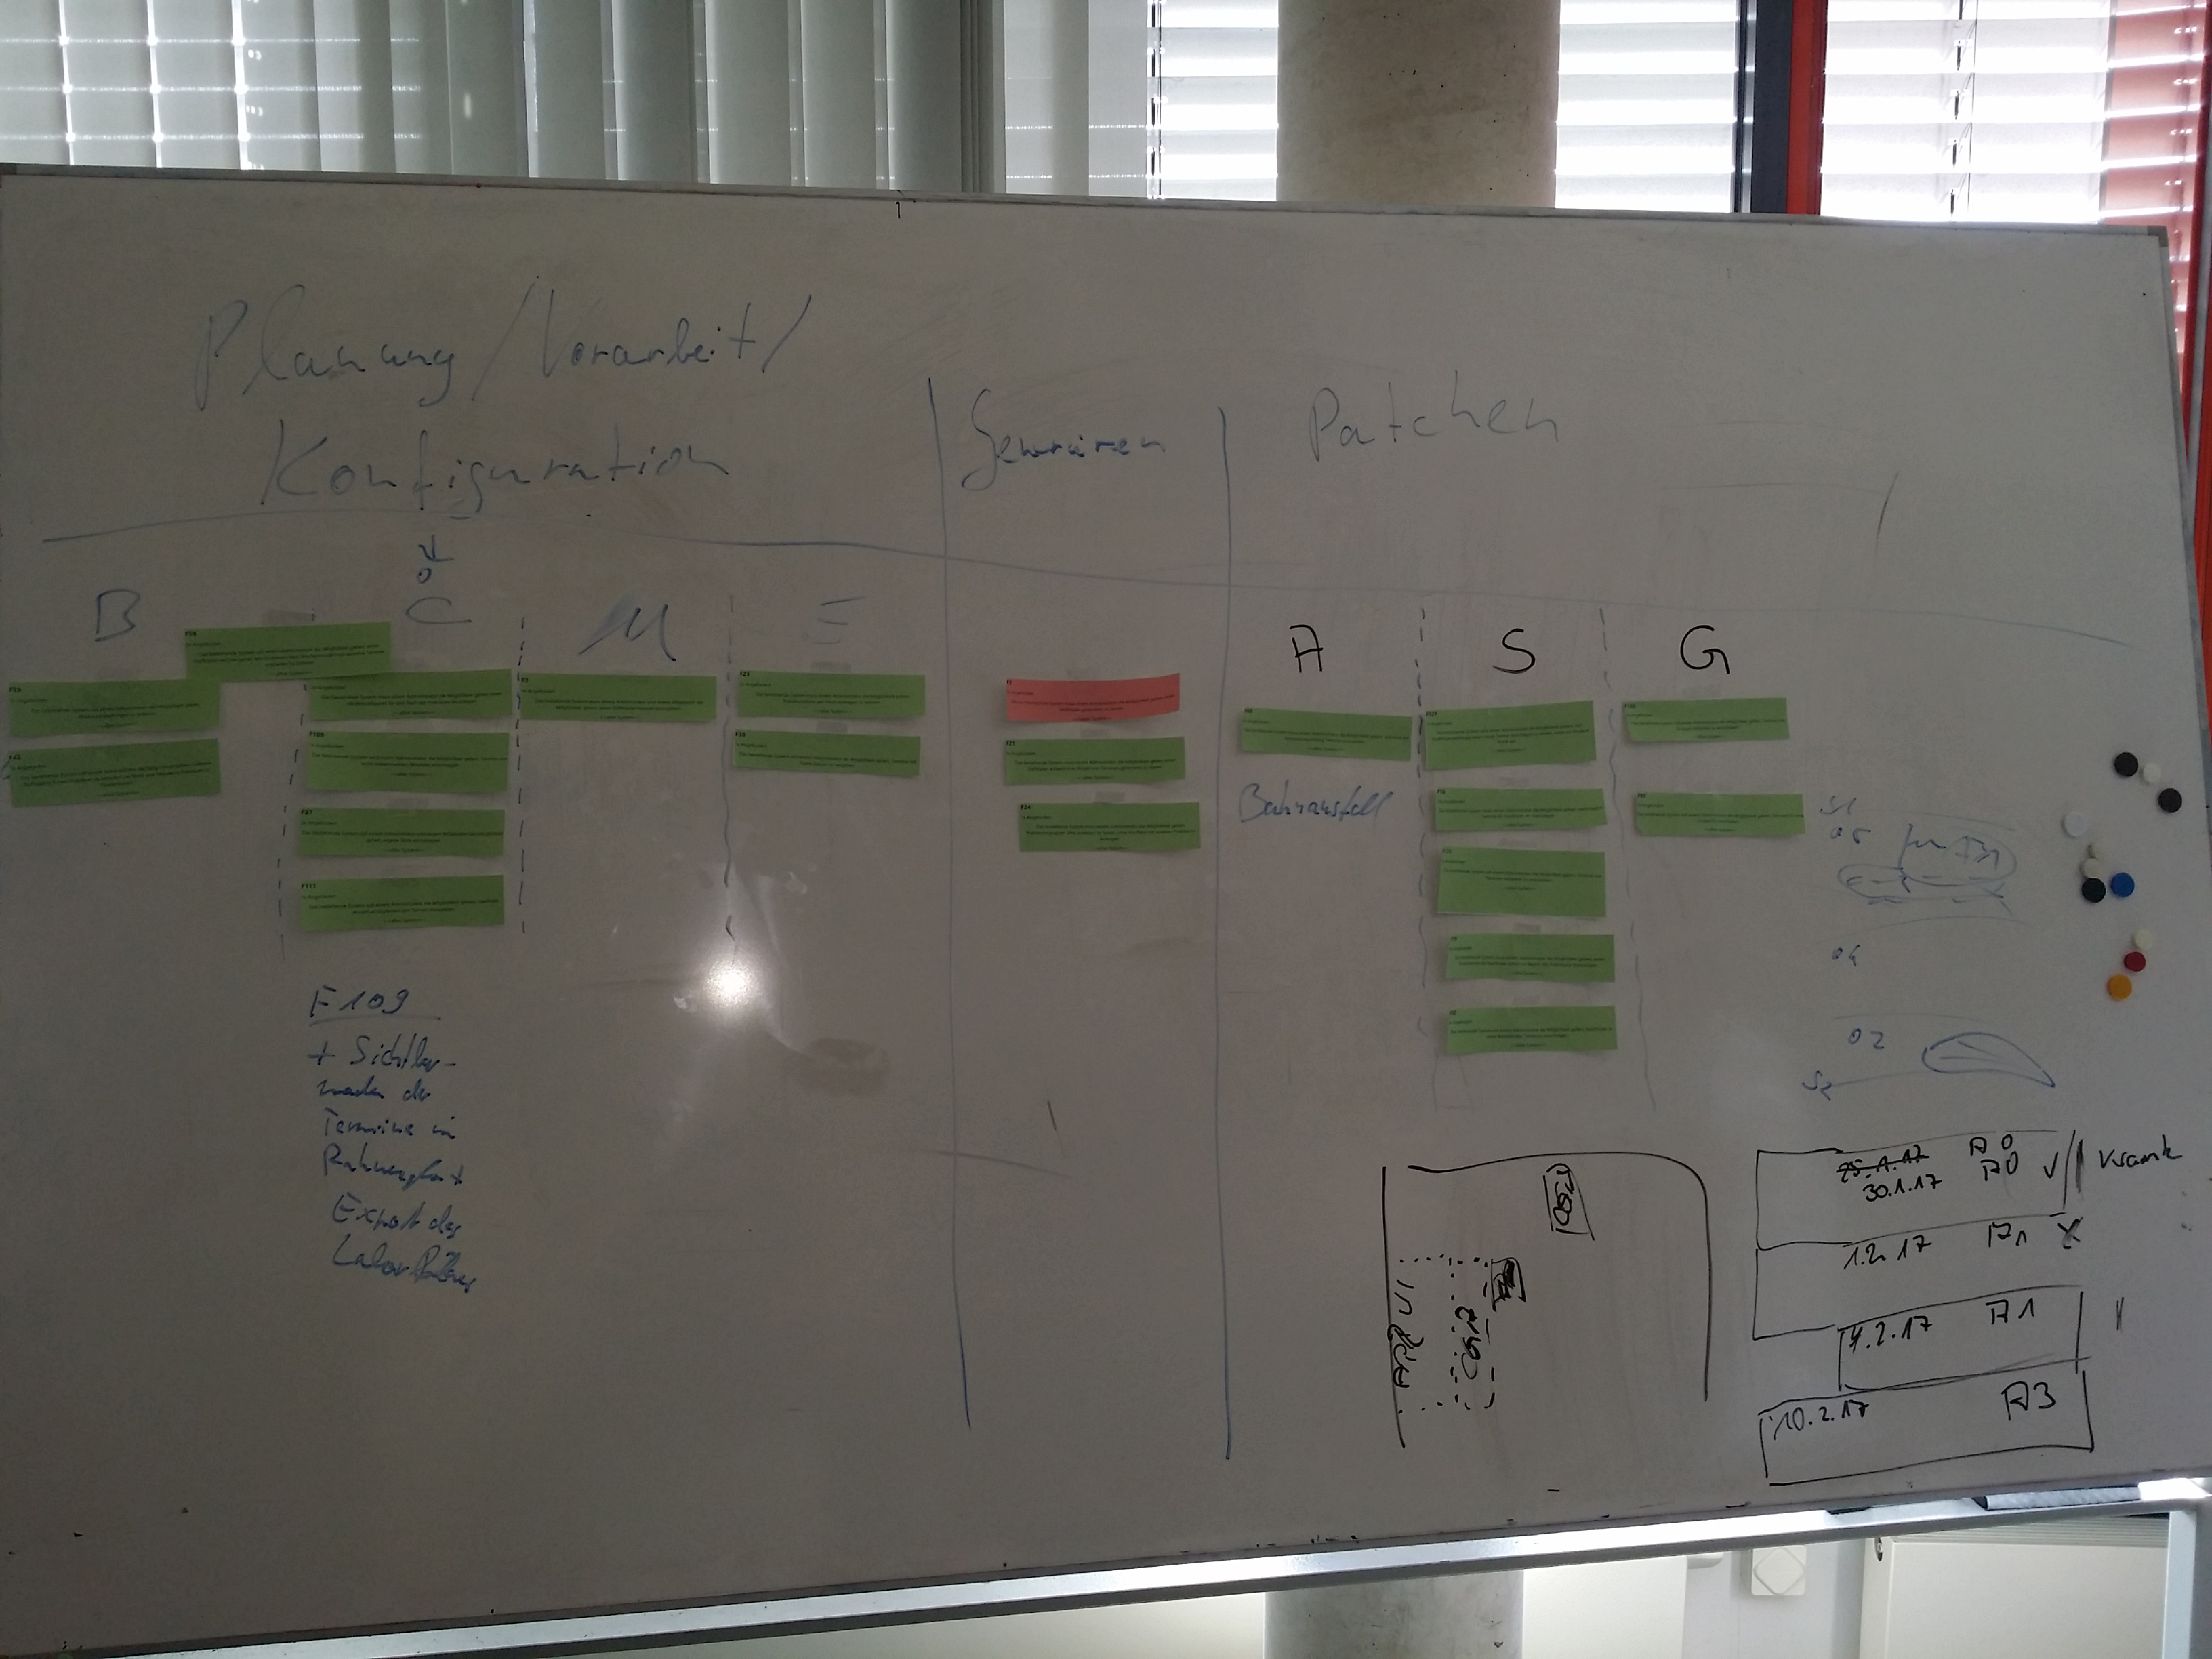
\includegraphics[width=\textwidth]{images/zweitegruppen.pdf}
\centering 
\captionabove[Gruppeneinteilung dritter \& vierter Ebene]{Gruppeneinteilung dritter \& vierter Ebene\footnotemark} 
\end{figure}
\footnotetext{Ein Bild von der Gruppeneinteilung auf dritter \& vierter Ebene an einem Whiteboard} 

Es wurde zwischen drei Ablaufphasen unterschieden, welche anschließend in weitere Teilgruppen aufgeteilt wurden.

\begin{enumerate}
\item Planung/Vorarbeit/Konfiguration
\begin{enumerate}
\item B => Blockpraktika
\item C => aktuelles Schema
\item M => manuelle Eingabe
\item F => flexible Eingaben
\end{enumerate}
\item Generieren
\item Patchen
\begin{enumerate}
\item A => betrifft alle
\item M => betrifft Studenten
\item G => betrifft Gruppen
\end{enumerate}
\end{enumerate}

Nach dieser Gruppierung sind die Anforderungen so sortiert, dass man die einzelnen Gruppen als Arbeitsschritte abarbeiten kann. Auch wurden im Laufe dieses Verfahrens neue Anforderungen aufgedeckt, die entweder aus der Sicht der Entwickler notwendig waren oder andere Anforderungen detaillieren. \\[1em]

Dieses Vorgehen wiederholt sich für alle Gruppen auf zweiter Ebene, sobald die Entwicklung des \ac{LWM}s so fortgeschritten ist, dass die nächsten Anforderungen implementiert werden können. 

\subsection{Priorisierung}
\label{subsec:priorisierung}

Die Priorisierung der Anforderungen ist notwendig, um erkennen zu können, wie wichtig eine Anforderung für die Zufriedenheit \textbf{aller} Stakeholder ist. Zudem wird diese Priorität nach der Aufwandsschätzung dazu genutzt, über die Umsetzungsreihenfolge der Anforderungen zu entscheiden.\\

Eine erste Priorisierung wurde nach der Gruppierung auf zweiter Ebene durchgeführt und wurde in Prozent angegeben. Dabei ist diese Zahl wie folgt zu interpretieren:
\begin{description}
\item $100\% \rightarrow$ \textbf{Alle} Stakeholder haben diese Anforderung als \textbf{Basisfaktor} bestimmt
\item $0\% \rightarrow$ \textbf{Kein} Stakeholder hat diese Anforderung erhoben
\end{description}

Für die Berechnung dieses Wertes wurde den einzelnen Kano-Faktoren und der Stimme eines Stakeholders (Vote) ein Wert und ein Variablen-Name zugewiesen:

\begin{description}
\item $ bap \rightarrow$ Basis-Faktor $\rightarrow$ 9
\item $ lp \rightarrow$ Leistungs-Faktor $\rightarrow$ 6
\item $ bep \rightarrow$ Begeisterungs-Faktor $\rightarrow$ 3
\item $ vp \rightarrow$ Vote $\rightarrow$ 1
\end{description}

Des Weiteren werden folgende Parameter benötigt:
\begin{description}
\item $ v \rightarrow$ die Votes der Anforderung
\item $ m \rightarrow$ die maximalen Votes die für eine Anforderung abgegeben wurden
\item $ p \rightarrow$ die Priorität in \%
\end{description}

Die Formel sieht dann wie folgt aus:
$$ p = \frac{v * vp + <bap|lp|bep>}{m*vp + bap}$$

Nachdem die Aufwandsschätzung abgeschlossen war, konnte mit dem dort geschätzten Wert und der Priorität deutlich gemacht werden, wie die Anforderung im Laufe der Entwicklung zu interpretieren ist.\\

Um die weitere Berechnung verstehen zu können, ist es wichtig zu wissen, dass die Komplexität einer Anforderung in Story-Points geschätzt wurde. Hierbei bedeuten 10 Story-Points, dass die Anforderung einen hohen Implementierungsaufwand mit sich bringt und 1 Story-Point, dass die Implementierung dieser am wenigsten komplex ist.\\

Das Prinzip dieser Interpretation wird mit der Abbildung \ref{fig:erklärung} deutlich.


\begin{figure}[!htb]
		\includegraphics[width=\textwidth]{images/ergebnis.pdf}
\centering 
\captionabove[Erklärung der Anforderungsauswertung]{Erklärung der Anforderungsauswertung\footnotemark} 
  \label{fig:erklärung}
\end{figure}
\footnotetext{Erklärung der Anforderungsauswertung anhand eines Beispiels} 

Auf Abbildung \ref{fig:erklärung} ist zu erkennen, dass die Anforderung \textit{F3} zwar einen hohen Implementierungsaufwand bedeutet, diese allerdings eine Stakeholder-Priorität von 90\% aufweist. Dagegen hat \textit{F5} nur eine Priorität von 20\%, jedoch ist diese auch wesentlich einfacher erfüllbar. Diese beiden Anforderungen haben also in erster Linie keine hohe Priorität bei der Entwicklung. \textit{F4} weist von den abgebildeten Beispielen die schlechteste Bewertung auf. Diese ist, wenn überhaupt, erst ganz am Ende zu betrachten, wenn alle anderen Anforderungen erfüllt wurden. \textit{F1} hingegen ist sofort umzusetzen, da diese nicht nur von den meisten Stakeholdern als wichtig angesehen wurde, sondern auch relativ einfach zu implementieren ist. \\[1em]

Durch die Abarbeitung in dieser Reihenfolge können die wichtigsten Wünsche der Stakeholder am schnellsten erfüllt werden, deshalb wurde für die Anforderungen bei diesem Projekt auch ein solcher Wert berechnet. Wie die Berechnung als Formel aussieht, wird nachfolgend gezeigt. Doch vorher muss auch für diese Formel die Definition einiger Variablen geklärt werden:

\begin{description}
\item $ sp \rightarrow$ die Story-Points die der Anforderung bei der Aufwandsschätzung zugewiesen wurde
\item $ p \rightarrow$ die Priorität der Anforderung in \%
\item $ r \rightarrow$ das Ergebnis der Berechnungen. (Da für diese Variable kein passender Name gefunden werden konnte, wird diese ab jetzt auch weiterhin Ergebnis genannt)
\end{description}

Nun ist es es ohne Probleme möglich, die Formel zu verstehen:
$$r = 100-\sqrt{(sp-1)^{2}+(100-p)^{2}}$$
Der Kern dieser Formel ist der Satz des Pythagoras:
$$c^{2} = a^{2}+ b^{2} \rightarrow c = \sqrt{a^{2}+ b^{2}}$$
Hierbei ist $c$ unser Ergebnis $r$, $a$ sind die Story-Points $- 1$. \\

\textbf{Doch warum Story-Points $- 1$?}\\
Wie in Kapitel \ref{subsec:validation} (\nameref{subsec:validation}) beschrieben wurde, konnte im Vorfeld entschieden werden, ob eine Anforderung als \textit{"Erledigt"}, \textit{"Valide"} oder \textit{"Verworfen"} anzusehen ist. Bei der weiteren Auswertung sind erledigte oder verworfene Anforderungen kaum noch von Interesse, deshalb werden diese in der Berechnung nicht beachtet. Das hat zur Folge, dass eine Anforderung, welche in diese Berechnung mit einfließt, einen Mindestaufwand von einem Story-Point haben muss. Schließlich gibt es keine noch nicht implementierte Anforderung, deren Realisierung keinen Aufwand mit sich zieht.\\

Mit der Rechnung "Story-Points $- 1$" wurde also eine Normalisierung durchgeführt, um mit einem Story-Point und 100\% Priorität auch ein Ergebnis von 100\% zu erzielen, denn das ist das Beste was eine Anforderung haben kann. \\

Schließlich ist noch das $b$ zu betrachten. Dieses wird durch $100-p$ ersetzt, wobei $p$ die Priorität der Anforderung ist, welche ohne Berücksichtigung der Komplexität errechnet wurde. Warum diese Priorität von 100 abgezogen wird, erkennt man in Abbildung \ref{fig:erklärung100-p}.


\begin{figure}[!htb]
\centering 
		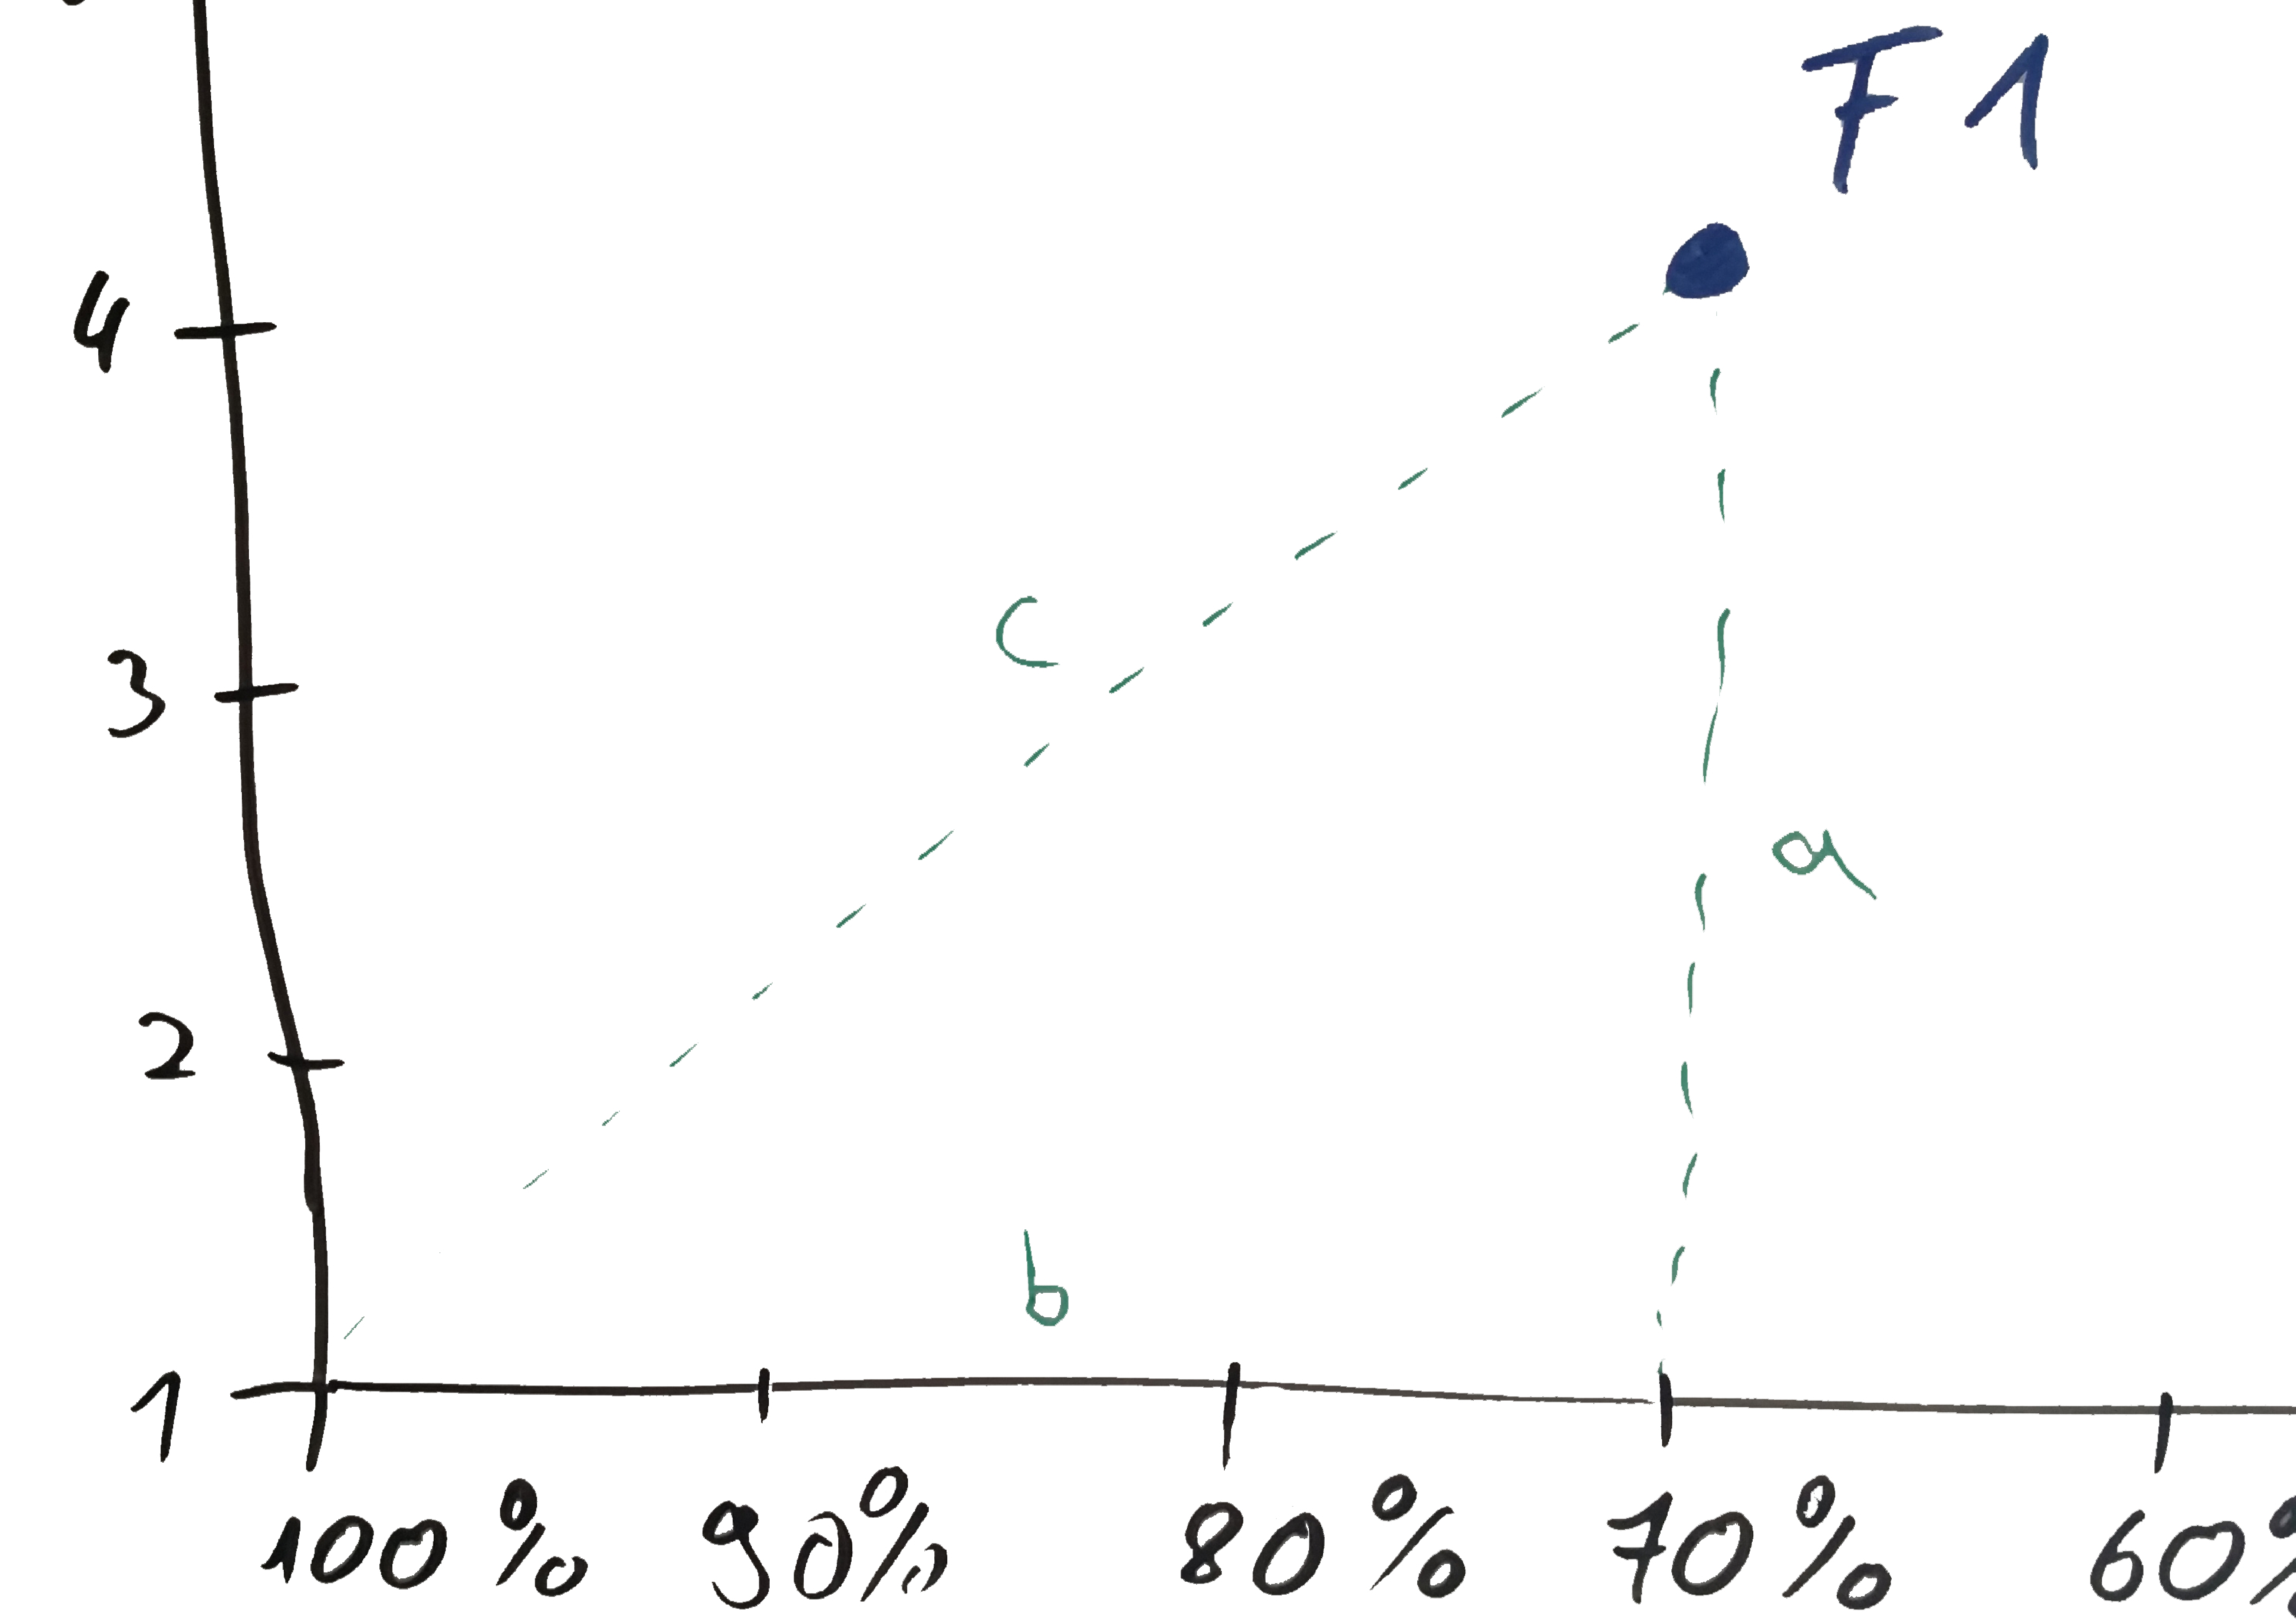
\includegraphics[width=0.5\textwidth]{images/100minusp.pdf}
\captionabove[Erklärung zur Rechnung 100 - p]{Erklärung zur Rechnung 100 - p\footnotemark} 
  \label{fig:erklärung100-p}
\end{figure}
\footnotetext{Eine Bild zur Erklärung für die Rechnung 100 - p bei der Priorisierung} 

Die y-Achse stellt die Skala der Priorität dar. Da laut der durchgeführten Rechnung $c$, also die Länge des Ortsvektor, die Bewertung der Anforderung darstellt, ist zu beachten, dass die y-Achse am Koordinatenursprung mit $100\%$ beginnt. Somit stellt eine Priorität von $70\%$ für $b$ nicht den Wert 70 dar, sondern $100-70$ also $30$.\\[1em]

Nachdem diese Berechnungen und somit die Bewertung der Anforderungen durchgeführt wurde, ist es dem Entwickler-Team möglich, die Anforderungen mit der richtigen Priorität zu implementieren.


\subsection{Aufwandsschätzung}
\label{subsec:aufwandsschätzung}

Bei der Aufwandsschätzung der ermittelten Anforderungen wurde sich aufgrund der agilen Entwicklung des \ac{LWM}s bewusst gegen die Anwendung der \ac{FPA} oder anderen klassischen Schätzmethoden entschieden. Statt dessen wurde an dieser Stelle von \ac{SP} Gebrauch gemacht. Der Grund dafür liegt neben dem hohen Aufwand einer Function-Point-Analyse in Erfahrungsberichten, die ebenfalls dazu raten.

\begin{quote}
\glqq Die Erfahrung (nicht nur der agilen Projektwelt) hat aber gezeigt, dass das vergleichende Schätzen in abstrakten Schätzmaßen zu deutlich schnelleren und besseren Ergebnissen führt.\grqq    \citep{AGIL1}
\end{quote}

Um eine Schätzung mit \acl{SP} durchführen zu können, werden die Anforderungen in eine \ac{US} aufgeteilt. Diese Storys bekommen anschließend Story-Points zugewiesen. In diesem Fall wurde ein Intervall von 1 - 10 festgelegt, wobei 1 für eine niedrige und 10 für eine sehr hohe Komplexität steht. Hierbei ist zu unterscheiden, dass, im Gegensatz zu klassischen Schätzverfahren, nicht der Aufwand sondern die Komplexität geschätzt wird. \\[1em]

Damit nun die Story-Points ordnungsgemäß zugewiesen werden konnten, wurde eine Anforderung rausgesucht, welche einen guten Mittelwert an Komplexität bedeutet. Dieser Anforderung wurden die ersten Punkte zugewiesen. Relativ zu dieser Schätzung wurde anschließend auch den übrigen Anforderungen ein Wert gegeben. Dieser Prozess wurde in einem Meeting mit dem Entwickler-Team vor Ort, im Zuge der detaillierteren Gruppierung, durchgeführt. Dazu haben sich die Entwickler von Frontend und Backend zu der Komplexität der jeweiligen Implementierung abgesprochen und sich auf eine Anzahl an Story-Points geeinigt. Dieses Verfahren kann man, genauso wie die Gruppierung, auch in weiteren Iterationen weiter verfeinern. Dazu werden diese \ac{US} wieder in kleinere aufgesplittet, welche wiederum \ac{SP} zugewiesen bekommen. Dieser Vorgang ist bei sehr groben \ac{US} zu empfehlen.\\[1em]

Die somit verteilten \ac{SP} konnten anschließend zur weiteren Priorisierung genutzt werden.

\chapter{Visualisierung der Ergebnisse}

Die ermittelten Anforderungen sollen, auch nach der Fertigstellung dieses Projekts, noch zur Orientierung bei der Entwicklung des \ac{LWM} dienen. Deshalb ist eine ordnungsgemäße und langfristige Speicherung der Anforderungen unumgänglich. Für die weitere Auswertung und Priorisierung ist es zudem notwendig, Berechnungen und Sortierungen mit den Anforderungen durchzuführen. \\[1em]

\section{Excel}
\begin{figure}[!htb]
		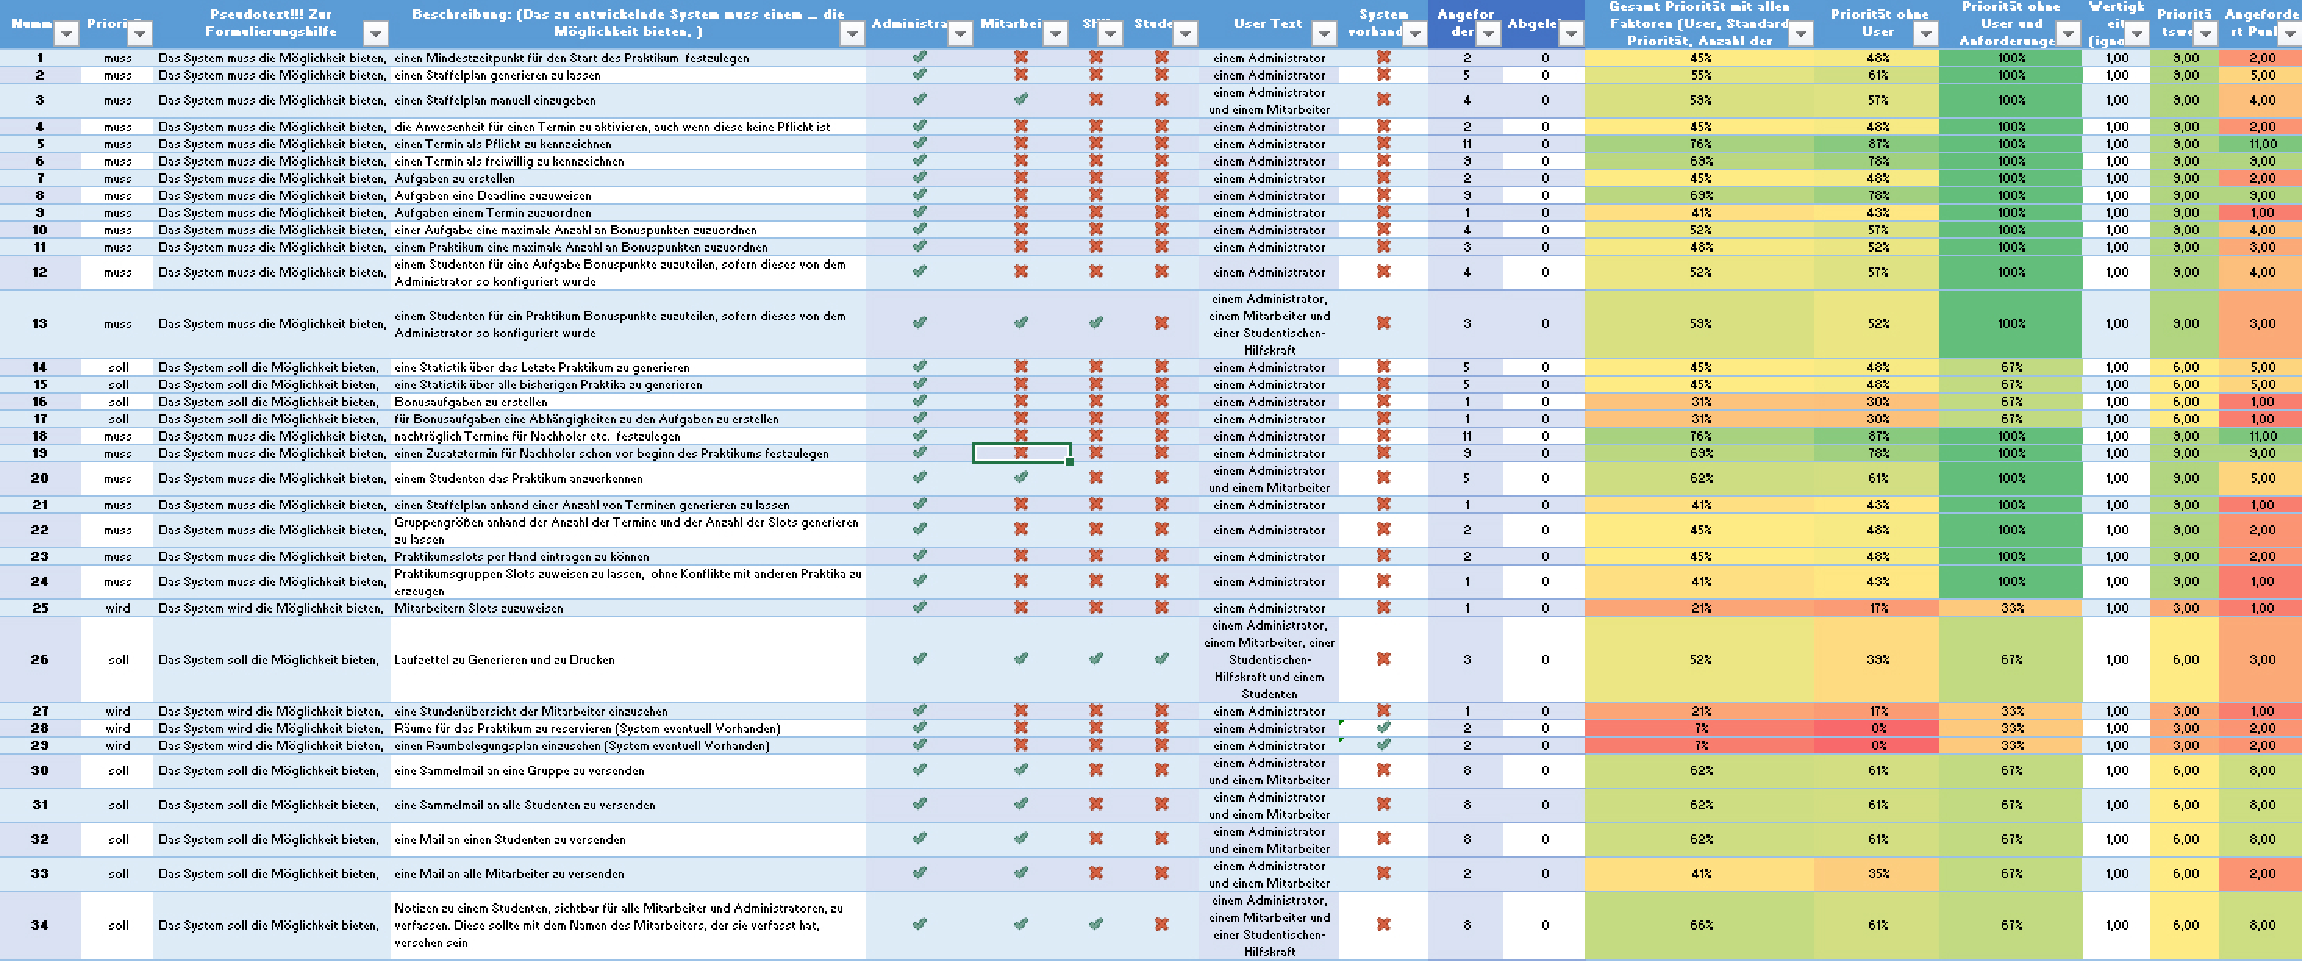
\includegraphics[width=\textwidth]{images/excel.pdf}
\centering 
\captionabove[Ausschnitt aus Excel]{Ausschnitt aus Excel\footnotemark} 
		\label{fig:excel}
\end{figure}
\footnotetext{Ein Ausschnitt aus der Dokumentation der Anforderungen in Excel} 
Der erste Ansatz war das Dokumentieren in Excel. Dort wurden (wie in Abbildung \ref{fig:excel} zu sehen) alle Anforderungen aufgenommen und erste Berechnungen der Prioritäten durchgeführt. Jedoch stellte sich im Laufe dieser Bearbeitung heraus, dass Excel nicht alle Funktionalitäten, die benötigt wurden, zufriedenstellend bereitgestellt. Zudem erfolgt die Speicherung der Daten in einer lokalen Datei, was deren aktive Nutzung von mehreren Beteiligten erschwert. Also wurde die Entscheidung getroffen ein Programm zum Verwalten der Daten zu entwickeln, damit dort alle notwendigen Funktionen nach belieben implementiert werden können.


\section{Website}

Eine einfache und effektive Lösung der Datenhaltung und -verarbeitung bot die Kombination einer Angular2-Webseite und einer MySQL-Datenbank. Durch vorherige Projekte bestand derzeit schon der Zugang zu einem Server und einer Datenbank, was diese Entscheidung stützte. Zudem ist die Erstellung einer Angular2-Webseite mit weniger Aufwand verbunden als ein Java-Programm, welches die andere Alternative gewesen wäre.\\

Durch diese Website bestand die Möglichkeit, auch ohne eine persönliche Zusammenkunft, mit dem Entwickler-Team einige Absprachen und Anpassungen durchzuführen. So konnten nicht nur dynamisch neue Anforderungen über ein perfekt dafür zurecht geschnittenes Interface hinzugefügt und mit den nötigen Informationen bestückt werden (Abbildung \ref{fig:erstellen}), sondern auch die Editierung dieser konnte, in die davon abhängigen Berechnungen, sofort mit einbezogen werden.\\

\begin{figure}[!htb]
		\includegraphics[width=.5\textwidth]{images/erstellen.pdf}
\centering 
\captionabove[Erstellen einer Anforderung]{Erstellen einer Anforderung\footnotemark} 
		\label{fig:erstellen}
\end{figure}
\footnotetext{Erstellen einer Anforderung mit einem eigens dafür konzipierten Interface} 


\subsection{Gruppen}
Ein weiterer Vorteil dieser Entscheidung war das einfache Gruppieren der Anforderungen. Um eine Anforderung einzufügen, wird diese direkt der jeweiligen Gruppe über den "Plus-Button" hinzugefügt. Sofern eine bestehende Anforderung in eine neue Gruppe geschoben werden soll, kann dies mittels "Drag and Drop" realisiert werden. Auch bei diesem Vorgang werden alle Folgeberechnungen angepasst. Auch die Übersicht dieser Gruppen ist in dieser App wesentlich besser als sie in Excel gewesen wäre (siehe Abbildung \ref{fig:gruppen}).

\begin{figure}[!htb]
		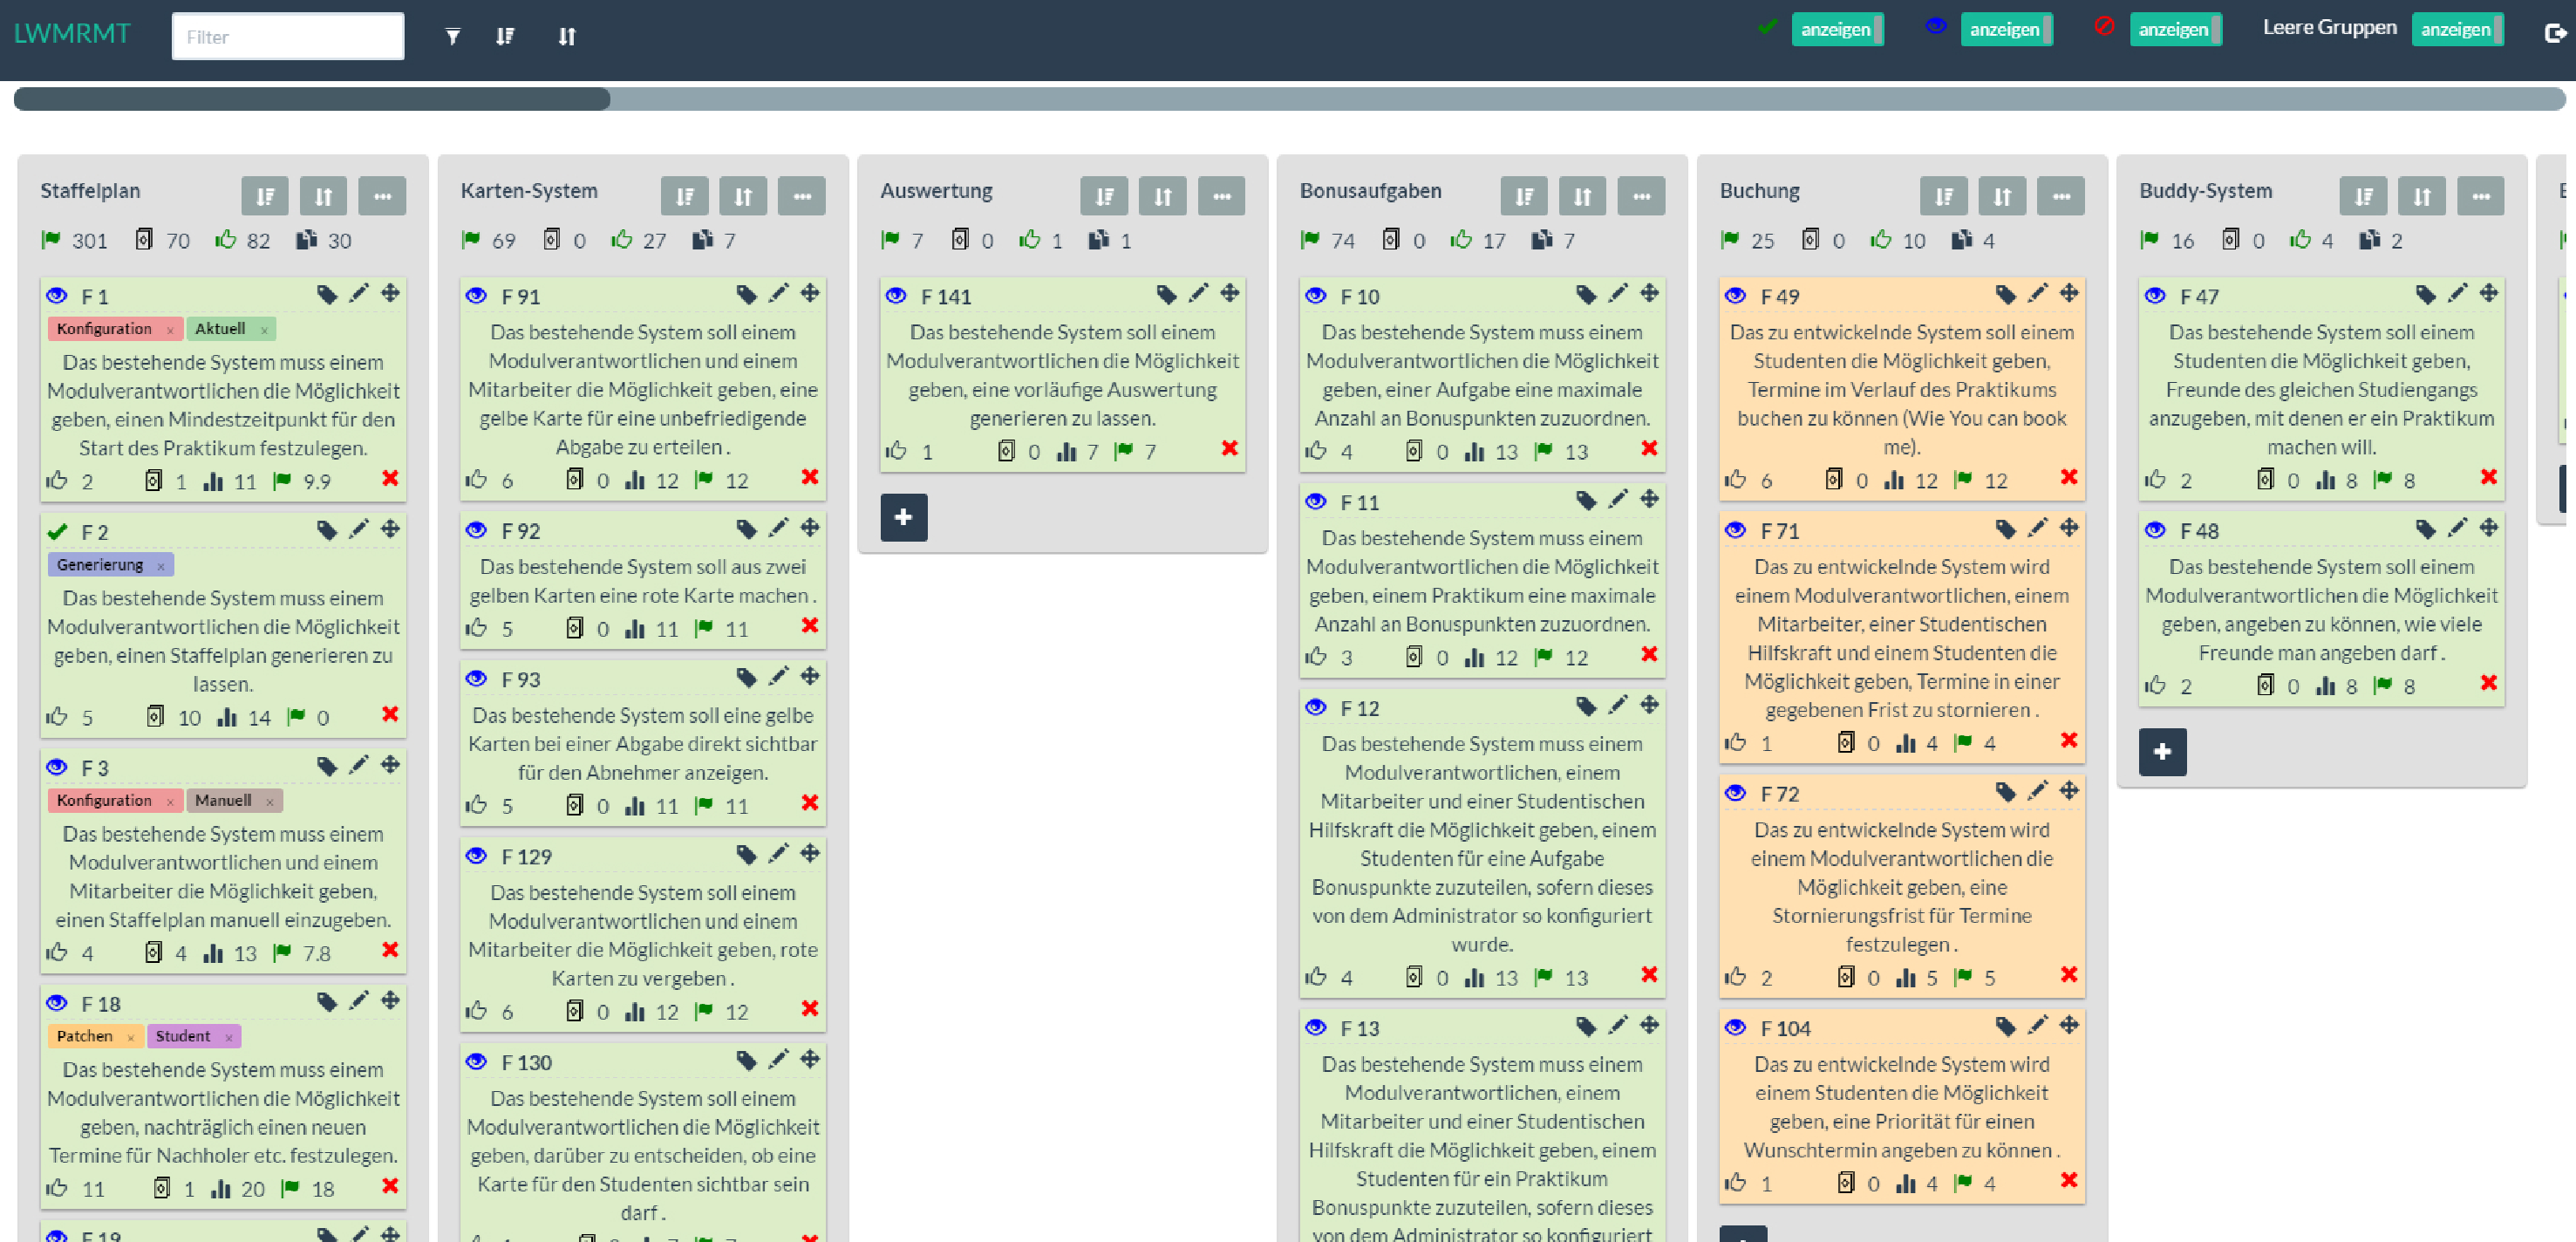
\includegraphics[width=\textwidth]{images/webseite.pdf}
\centering 
\captionabove[Ausschnitt der Webseite]{Ausschnitt der Webseite\footnotemark} 
\label{fig:gruppen}
\end{figure}
\footnotetext{Ein Ausschnitt aus der Dokumentation der Anforderungen mit der Webseite} 


\subsection{Labels}
Das Programm bietet zudem ein Interface, mit dem man Labels für eine Gruppe erstellen kann (Abbildung \ref{fig:labelerstellen}).

\begin{figure}[!htb]
		\includegraphics[width=.5\textwidth]{images/labelserstellen.pdf}
\centering 
\captionabove[Erstellen eines Labels]{Erstellen eines Labels\footnotemark} 
\label{fig:labelerstellen}
\end{figure}
\footnotetext{Das Erstellen eines Labels in einer Gruppe über das User-Interface}

Diese können anschließend den Anforderungen dieser Gruppe zugeordnet werden (Abbildung \ref{fig:labelzuordnen}). 

\begin{figure}[!htb]
		\includegraphics[width=.25\textwidth]{images/labelzuordnen.pdf}
\centering 
\captionabove[Zuordnen eines Labels]{Zuordnen eines Labels\footnotemark} 
\label{fig:labelzuordnen}
\end{figure}
\footnotetext{Zuordnen eines Labels zu einer Anforderung mit dem User-Interface} 

\subsection{Informationen}
Die Anforderungen selbst bieten alle nötigen Informationen auf einem Blick, wie in Abbildung \ref{fig:anforderung} zu erkennen ist.

\begin{figure}[!htb]
		\includegraphics[width=.5\textwidth]{images/anforderung.pdf}
\centering 
\captionabove[Eine Anforderung im User-Interface]{Eine Anforderung im User-Interface\footnotemark} 
\label{fig:anforderung}
\end{figure}
\footnotetext{Die Detail-Ansicht einer Anforderung im User-Interface}

Hier sind nicht nur die zugewiesenen Labels zu erkennen, sondern diese Karte zeigt alle Informationen über diese Anforderung. 

\begin{figure}[!htb]
		\includegraphics[width=0.05\textwidth]{images/thumbs.pdf}
	\textit{Die Anzahl der Votes}
\end{figure}
\vspace{-15pt}
\begin{figure}[!htb]
		\includegraphics[width=0.05\textwidth]{images/cards.pdf}
	\textit{Die Anzahl der Story-Points}
\end{figure}
\vspace{-15pt}
\begin{figure}[!htb]
		\includegraphics[width=0.05\textwidth]{images/stats.pdf}
	\textit{Die Priorität in \%}
\end{figure}
\vspace{-15pt}
\begin{figure}[!htb]
		\includegraphics[width=0.05\textwidth]{images/flag.pdf}
	\textit{Das Ergebnis in \%}
\end{figure}
\vspace{-15pt}
\begin{figure}[!htb]
		\includegraphics[width=0.05\textwidth]{images/eye.pdf}
	\textit{Der Status der Anforderung, in diesem Fall "Valide"}
\end{figure}
\vspace{-15pt}
\begin{figure}[!htb]
		\includegraphics[width=0.05\textwidth]{images/ok.pdf}
	\textit{Der Status der Anforderung, wenn sie "Erledigt" ist}
\end{figure}
\vspace{-15pt}
\begin{figure}[!htb]
		\includegraphics[width=0.05\textwidth]{images/ban.pdf}
	\textit{Der Status der Anforderung, wenn sie "Verworfen" ist}
\end{figure}

\pagebreak
Auch eine Gruppe hat alle Informationen direkt ersichtlich, die dort verwendeten Zeichen haben die gleiche Bedeutung wie bei einer Anforderung, mit dem Unterschied, dass diese Daten sich aus den Anforderungen der Gruppe zusammensetzen (Abbildung \ref{fig:gruppeninfo}).

\begin{figure}[!htb]
		\includegraphics[width=.5\textwidth]{images/groupinfo.pdf}
\centering 
\captionabove[Gruppeninformationen]{Gruppeninformationen\footnotemark} 
\label{fig:gruppeninfo}
\end{figure}
\footnotetext{Die Informationen einer Gruppe im User-Interface}

\begin{figure}[!htb]
		\includegraphics[width=0.05\textwidth]{images/flag.pdf}
	\textit{Der Durchschnitt aller Ergebnisse der beinhalteten Anforderungen}
\end{figure}
\vspace{-15pt}
\begin{figure}[!htb]
		\includegraphics[width=0.05\textwidth]{images/cards.pdf}
	\textit{Die Summe aller Story-Points der beinhalteten Anforderungen}
\end{figure}
\vspace{-15pt}
\begin{figure}[!htb]
		\includegraphics[width=0.05\textwidth]{images/thumbs.pdf}
	\textit{Die Summe aller Votes der beinhalteten Anforderungen}
\end{figure}
\vspace{-15pt}
\begin{figure}[!htb]
		\includegraphics[width=0.05\textwidth]{images/files.pdf}
	\textit{Die Anzahl beinhalteten Anforderungen}
\end{figure}

\subsection{Filter/Suche}
Neben diesen Informationen stehen zahlreiche Filter-Methoden und Sortierungs-Methoden zur Verfügung, welche eine Visualisierung über Graphen oder Charts überflüssig machen, da durch diese Methoden alles Nötige ersichtlich ist. Welche Methoden das sind, wird mit Abbildung \ref{fig:header} erklärt.  

\begin{figure}[!htb]
		\includegraphics[width=.5\textwidth]{images/filter.pdf}
\centering 
\captionabove[Filter-Methoden]{Filter-Methoden\footnotemark} 
\label{fig:header}
\end{figure}
\footnotetext{Ein Ausschnitt von dem Header des User-Interface mit allen Filter-Methoden}

Hierbei kann eingestellt werden, in welchen Elementen gesucht werden soll.
\begin{description}
\item Gruppen:\\
\textit{Hier wird in allen Gruppennamen gesucht}
\item Texte:\\
\textit{Hier wird in allen Texten, also in den Anforderungsbeschreibungen gesucht}
\item Id's:\\
\textit{Bezieht die Id´s der Anforderungen mit ein}
\item Labels:\\
\textit{Bezieht die Labels mit ein, welche den Anforderungen zugeordnet wurden}
\end{description}

Zudem kann nach mehreren Texten gleichzeitig gesucht werden. Dazu wird für eine \textit{"und"} Verknüpfung ein \textit{", "} und für eine \textit{"oder"} Verknüpfung ein \textit{"; "} verwendet. Hierbei ist zu beachten, dass eine \textit{"und"} Verknüpfung immer höher priorisiert wird. So könnte ein Filter-String wie folgt aussehen:

\begin{quote}
\textit{"Staffelplan, Generierung; Stat, 14"}
\end{quote}

Nach dem deaktivieren des Texte-Filters sieht das Ergebnis wie in Abbildung \ref{fig:filterergebnis} aus.

\begin{figure}[!htb]
		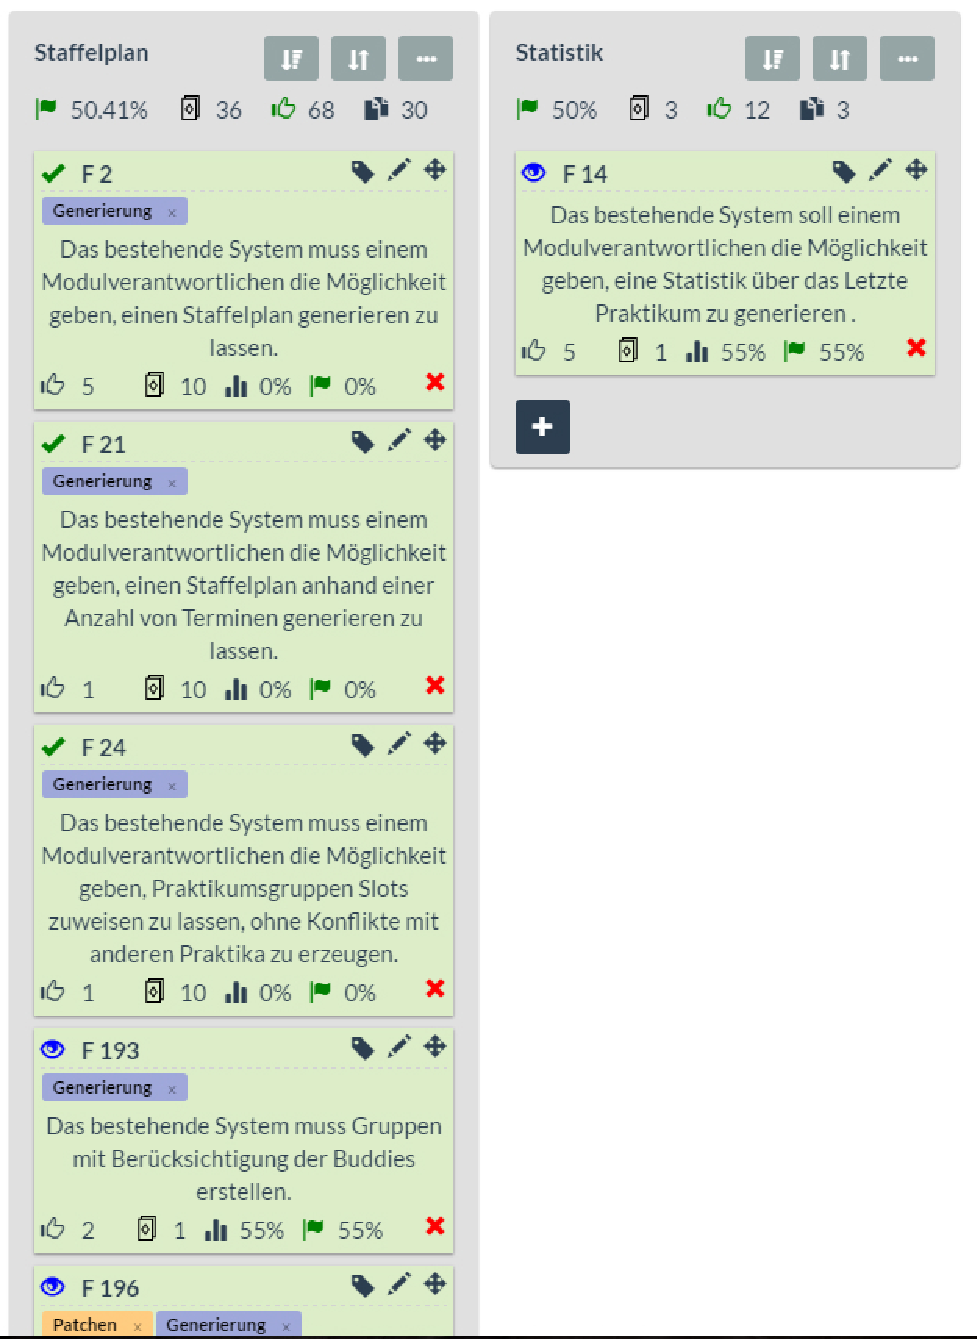
\includegraphics[width=.5\textwidth]{images/filterergebnis.pdf}
\centering 
\captionabove[Filter-Ergebnis]{Filter-Ergebnis\footnotemark} 
\label{fig:filterergebnis}
\end{figure}
\footnotetext{Das Ergebnis der Filterung nach \textit{"Staffelplan, Generierung; Stat, 14"}}

\subsection{Sortierung}
Durch die Kombination der Filter-Methoden mit den Sortierungs-Methoden können beinahe alle möglichen Anfragen erzeugt werden. Auch hier stehen einige Auswahlmöglichkeiten zur Verfügung. Die Abbildungen \ref{fig:sortgruppe}, welche die Sortierung in einer Gruppe anzeigt und \ref{fig:sortgesamt}, auf der die Möglichkeiten für die Sortierung aller Gruppen zu sehen ist, sollten selbsterklärend sein.

\begin{figure}[!htb]
		\includegraphics[width=.25\textwidth]{images/sortierunggruppe.pdf}
\centering 
\captionabove[Sortierung innerhalb einer Gruppe]{Sortierung innerhalb einer Gruppe\footnotemark} 
\label{fig:sortgruppe}
\end{figure}
\footnotetext{Ein Ausschnitt des User-Interface, auf dem die Möglichkeiten zur Sortierung innerhalb einer Gruppe zu sehen sind}

\begin{figure}[!htb]
		\includegraphics[width=.25\textwidth]{images/sortierunggesamt.pdf}
\centering 
\captionabove[Sortierung gesamt]{Sortierung gesamt\footnotemark} 
\label{fig:sortgesamt}
\end{figure}
\footnotetext{Ein Ausschnitt des User-Interface, auf dem die Möglichkeiten zur Sortierung aller Gruppen zu sehen sind}

\subsection{Sichtbarkeit}
Da sich die Filterung nur auf die Anforderungen selbst bezieht kann es sein, dass nach einer Filterung die Gruppen, welche keine zutreffenden Anforderungen beinhalten, zwar leer sind, jedoch trotzdem angezeigt werden. Dies hat den Grund, dass es durchaus sein kann, dass nach der Filterung eine der gefilterten Anforderungen in eine dann leere Gruppe verschoben werden soll. Ist dies nicht erwünscht besteht die Möglichkeit auch dies zu deaktivieren. Auch die Sichtbarkeit der Anforderungen mit einem bestimmten Status kann eingestellt werden, wie auf Abbildung \ref{fig:sichtbarkeit} zu erkennen ist.

\begin{figure}[!htb]
		\includegraphics[width=\textwidth]{images/sichtbarkeit.pdf}
\centering 
\captionabove[Sichtbarkeit]{Sichtbarkeit\footnotemark} 
\label{fig:sichtbarkeit}
\end{figure}
\footnotetext{Ein Ausschnitt des User-Interface, auf dem die Möglichkeiten zur Verstellung der Sichtbarkeit zu sehen sind}

All diese Funktionen haben wesentlich zur Bearbeitung und Auswertung der Anforderungen beigetragen und werden es auch noch in Zukunft tun. Diese Web-Anwendung steht unter der Adresse \textit{\href{http://www.req.herborn-software.com}{req.herborn-software.com}} zur Verfügung. Der Login wird nur auf Anfrage vom Verfasser dieses Dokuments vergeben, da Änderungen der Anforderungen direkte Auswirkung auf den Datenbestand haben, und diese Informationen auch nach diesem Projekt weiter verwendet werden.

\nomenclature{Epic}{Die Beschreibung einer Anforderung an eine Software auf einer hohen Abstraktionsebene.\vspace{4mm}}

\chapter{Ergebnisse}

Die Auflistung von 150 Anforderungen wäre an dieser Stelle unangebracht, weshalb hier nur die Top-10 der wichtigsten Anforderungs-Gruppe \textit{"Staffelplan"} aufgeführt werden. Diese Auflistung sollte genug über die Ergebnisse dieser Arbeit aussagen.\\


\begin{minipage}[t]{.5\textwidth}
	\centering
   		\textbf{1. Platz}\\
   		\vspace{16pt}
		\includegraphics[width=\textwidth]{images/1.pdf}
\end{minipage}
\begin{minipage}[t]{.5\textwidth}
	\centering
   		\textbf{2. Platz}\\
   		\vspace{16pt}
		\includegraphics[width=\textwidth]{images/2.pdf}
\end{minipage}



\begin{minipage}[t]{.5\textwidth}
	\centering
   \vspace{16pt}
   		\textbf{3. Platz}\\
   		\vspace{16pt}
		\includegraphics[width=\textwidth]{images/3.pdf}
\end{minipage}
\begin{minipage}[t]{.5\textwidth}
	\centering
   \vspace{16pt}
   		\textbf{4. Platz}\\
   		\vspace{16pt}
		\includegraphics[width=\textwidth]{images/4.pdf}
\end{minipage}



\begin{minipage}[t]{.5\textwidth}
	\centering
   \vspace{16pt}
   		\textbf{5. Platz}\\
   		\vspace{16pt}
		\includegraphics[width=\textwidth]{images/5.pdf}
\end{minipage}
\begin{minipage}[t]{.5\textwidth}
	\centering
   \vspace{16pt}
   		\textbf{6. Platz}\\
   		\vspace{16pt}
		\includegraphics[width=\textwidth]{images/6.pdf}
\end{minipage}



\begin{minipage}[t]{.5\textwidth}
	\centering
   \vspace{16pt}
   		\textbf{7. Platz}\\
   		\vspace{16pt}
		\includegraphics[width=\textwidth]{images/7.pdf}
\end{minipage}
\begin{minipage}[t]{.5\textwidth}
	\centering
   \vspace{16pt}
   		\textbf{8. Platz}\\
   		\vspace{16pt}
		\includegraphics[width=\textwidth]{images/8.pdf}
\end{minipage}



\begin{minipage}[t]{.5\textwidth}
	\centering
   \vspace{16pt}
   		\textbf{9. Platz}\\
   		\vspace{16pt}
		\includegraphics[width=\textwidth]{images/9.pdf}
\end{minipage}
\begin{minipage}[t]{.5\textwidth}
	\centering
   \vspace{16pt}
   		\textbf{10. Platz}\\
   		\vspace{16pt}
		\includegraphics[width=\textwidth]{images/10.pdf}
\end{minipage}

\chapter*{Fazit}
\addcontentsline{toc}{chapter}{Fazit}

Dieses Projekt hatte das Ziel, Anforderungen für das \ac{LWM} zur Verbesserung der Nutzbarkeit und Erweiterung des Nutzerkreises zu ermitteln. Dazu wurden Interviews mit den potentiellen neuen Usern und den bisherigen Nutzern durchgeführt. Die dort entstandenen Ergebnisse wurden zu einer soliden Grundlage für die weitere Entwicklung des Tools aufgearbeitet.\\

Die in dieser Arbeit hervorgebrachten Ergebnisse sollten mit Hilfe weiterer Methoden, wie dem Brainstorming oder anderen, erweitert und verfeinert werden. Zwar sind alle Entwickler des \ac{LWM} selbst Studenten, dennoch reichte das nicht aus, um wirklich alle Anforderungen der Studenten abzudecken. Hierzu hätte man, sofern es Zeitlich möglich gewesen wäre, mit Fragebögen auch die Studenten an dieser Anforderungserhebung teilnehmen lassen können.\\

Diese Arbeit bringt hervor, dass bei vielen Modulen, die dieses Tool noch nicht nutzen ein Interesse zur Nutzung vorhanden ist. Allerdings war dieses den Modulverantwortlichen bislang nicht bekannt, oder die benötigten Funktionen sind in der derzeitigen Anwendung noch nicht implementiert. Durch die Implementierung der hier ermittelten Anforderungen wäre es denkbar, auch diese Module als Nutzer zu gewinnen.\\

Des Weiteren stellte sich heraus, dass das Programm auch bei den aktuellen Nutzern teilweise Wünsche offen lässt, weshalb die Berücksichtigung der hier erlangten Erkenntnisse auch die Zufriedenheit der jetzigen Nutzer steigern könnte. \\

Durch diese Arbeit wird deutlich, dass die Anforderungsanalyse ein wichtiger Schritt in der Software-Entwicklung ist. Durch die sorgfältige Durchführung kann nicht nur die Usability einer Anwendung maßgeblich verbessert werden, sondern auch das Interesse bei einer viel größeren Nutzerzahl geweckt werden. Und gerade letzteres ist meistens der wichtigste Anreiz bei der Entwicklung einer Software.\\
Denn was ist schon eine Software ohne Nutzer?